% ===================================================================================================
\chapter{Results}
% ===================================================================================================

For each successful simulation, two coordinate dump files were produced, one containing the coordinates of the H and T atoms every 250 time steps ($2.5\cdot 10^{-4}$ ns) and another with the W atom coordinates every $5\cdot 10^5$ time steps (0.5 ns).
Since the motion of the defects themselves was practically negligible, the number of H and T bound to a defect could be determined by defining a geometric region in space around the defect and overlaying this region with each frame of the H-T dump file.

In practice, this was performed by parsing the dump files with a simple Fortran program, which checked whether each atom was located inside or outside the specified region and outputted the numbers of H and T in the defect as a functions of time.

% ----------------------------------------------------------------------------------
\section{Vacancies}
% ----------------------------------------------------------------------------------
In fig. (\ref{Fig:1Vac_results}) we can see the number of T and H atoms bound to the monovacany as a function of time, for three different temperatures. 
For comparison, the results of the monoisotopic, 'vacuum annealing', simulations are also shown. 

\begin{figure}[ht]
\begin{subfigure}{.5\textwidth}
  \centering
  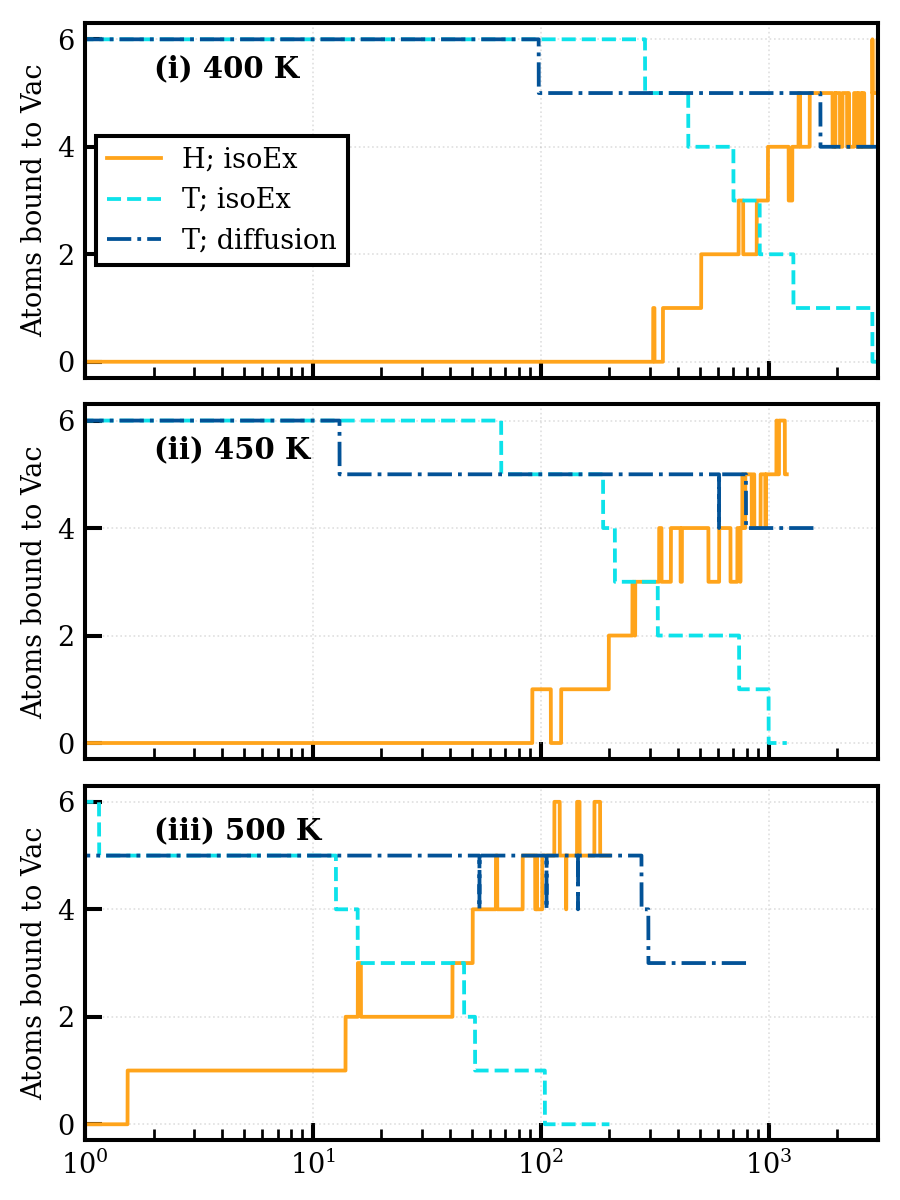
\includegraphics[width=0.99\textwidth]{1Vac_isoEx_HT_log.png}  
  \caption{Logarithmic time scale}
  %\label{fig:sub-first}
\end{subfigure}
\begin{subfigure}{.5\textwidth}
  \centering
  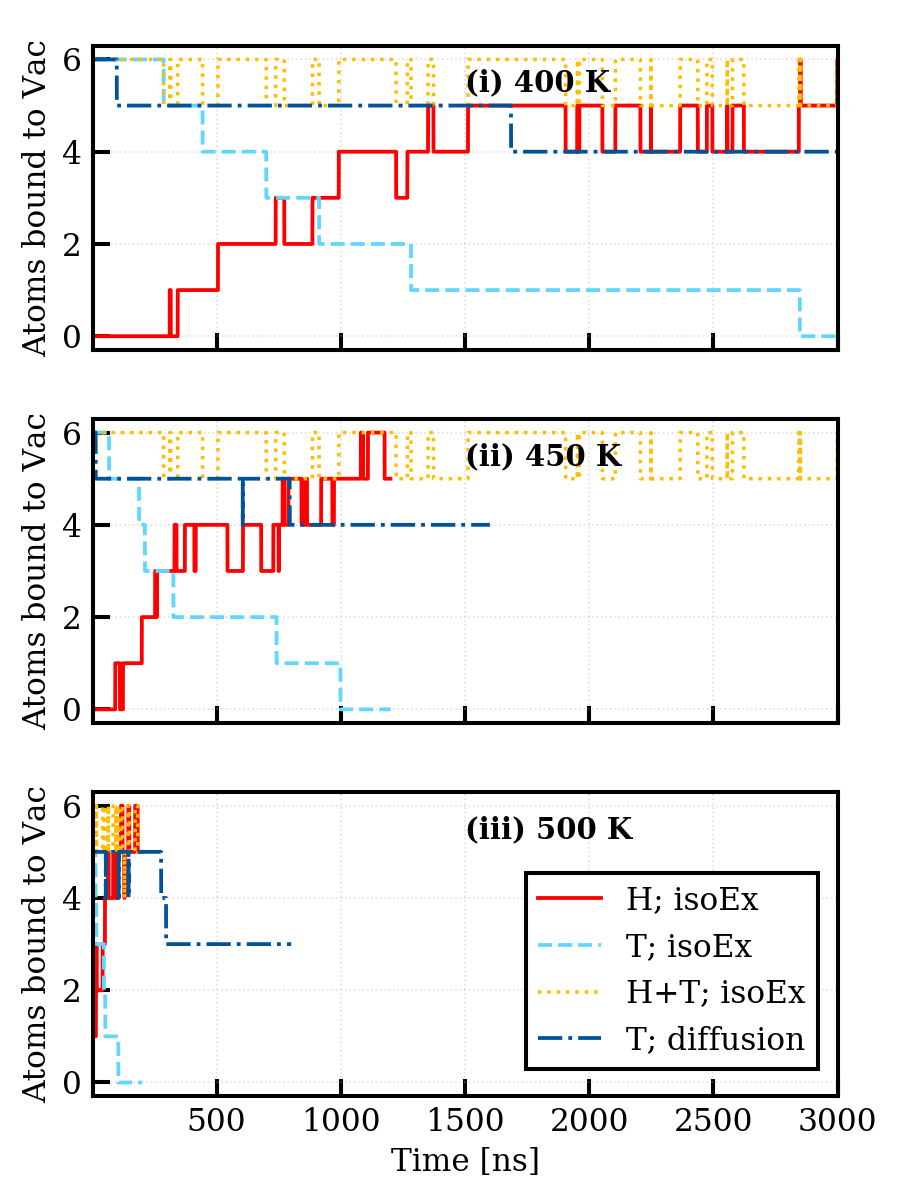
\includegraphics[width=0.99\textwidth]{1Vac_isoEx_HT.png}  
  \caption{Linear time scale}
  %\label{fig:sub-second}
\end{subfigure}
\caption{Number of H and T atoms in the monovacany for isotope exchange and diffusion simulations}
 \label{Fig:1Vac_results} 
\end{figure}


\begin{figure}[ht]
\begin{subfigure}{.5\textwidth}
  \centering
 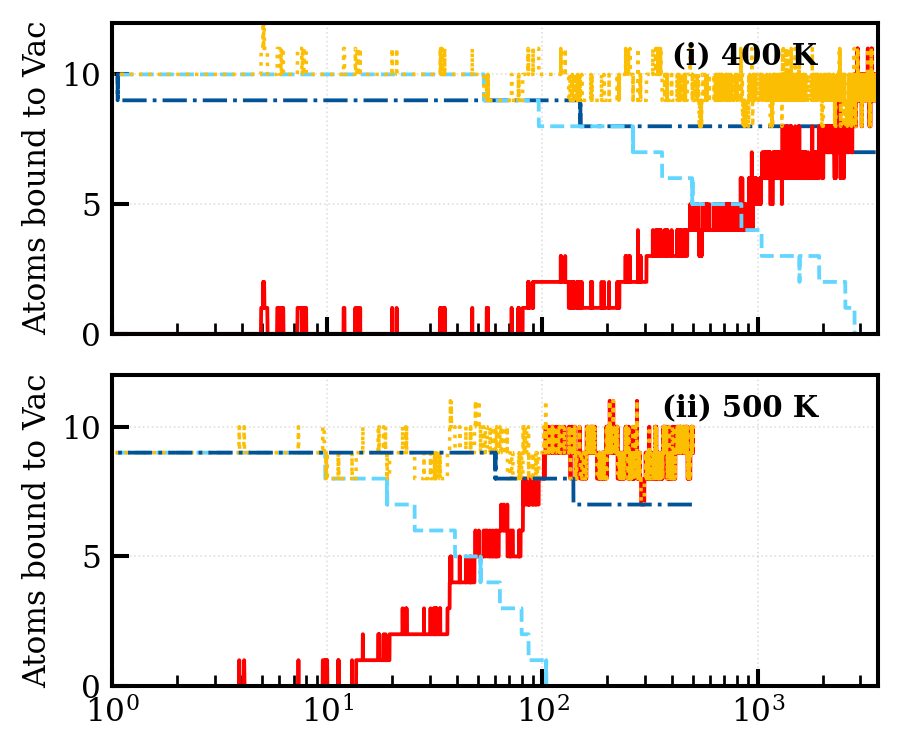
\includegraphics[width=0.99\textwidth]{2Vac_isoEx_HT_log.png}  
  \caption{Logarithmic time scale}
  %\label{fig:sub-first}
\end{subfigure}
\begin{subfigure}{.5\textwidth}
  \centering
  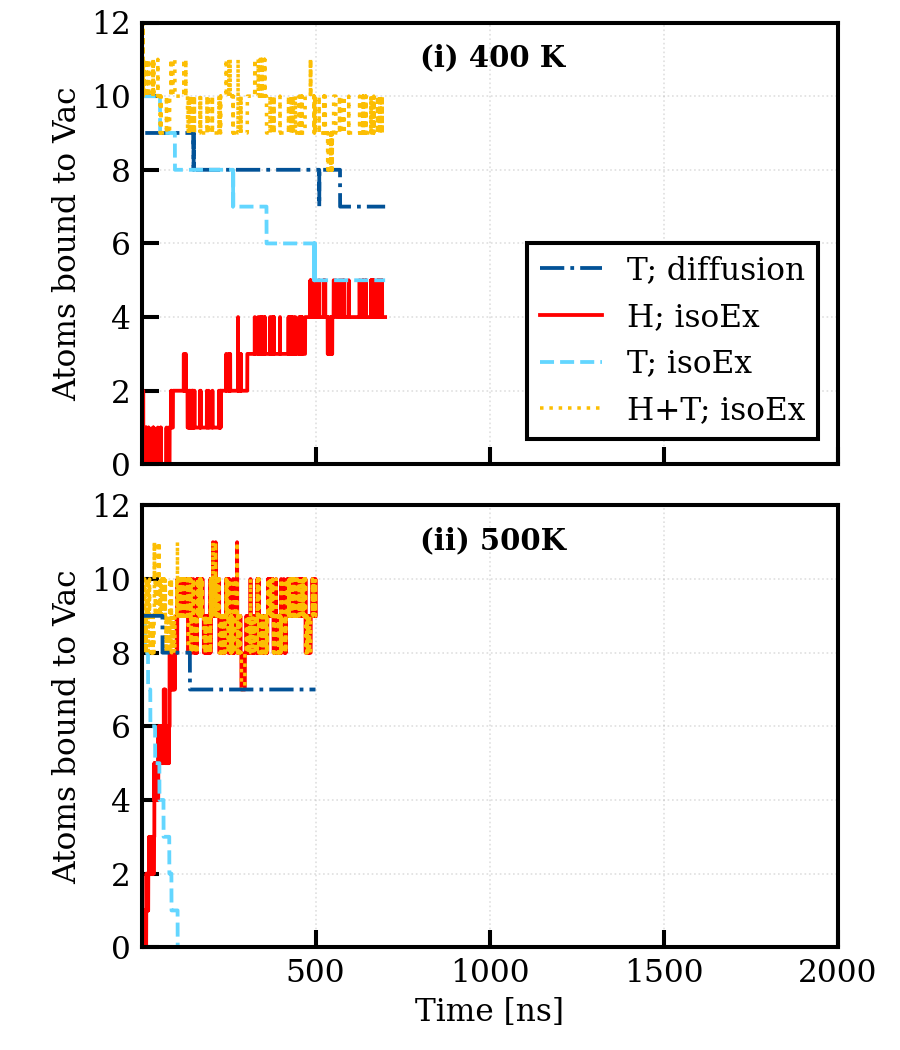
\includegraphics[width=0.99\textwidth]{2Vac_isoEx_HT.png}  
  \caption{Linear time scale}
  %\label{fig:sub-second}
\end{subfigure}
   \caption{Number of H and T atoms in the divacancy for isotope exchange and diffusion simulations}
   \label{Fig:2Vac_results} 
\end{figure}

From the figures \ref{Fig:1Vac_results} and \ref{Fig:2Vac_results} it is evident that the addition of T significantly increases the rate of T removal from both mono- and divacancies. 

Although to the potential gives smaller binding energy values for the hydrogen-vacancy interaction than DFT (Fig. \ref{Fig:Ebind1H_DFT}), the monoisotopic comparison simulations (Fig. \ref{Fig:1Vac_results}) clearly show that qualitative results are indeed valid.

\begin{figure}[!ht]
\center
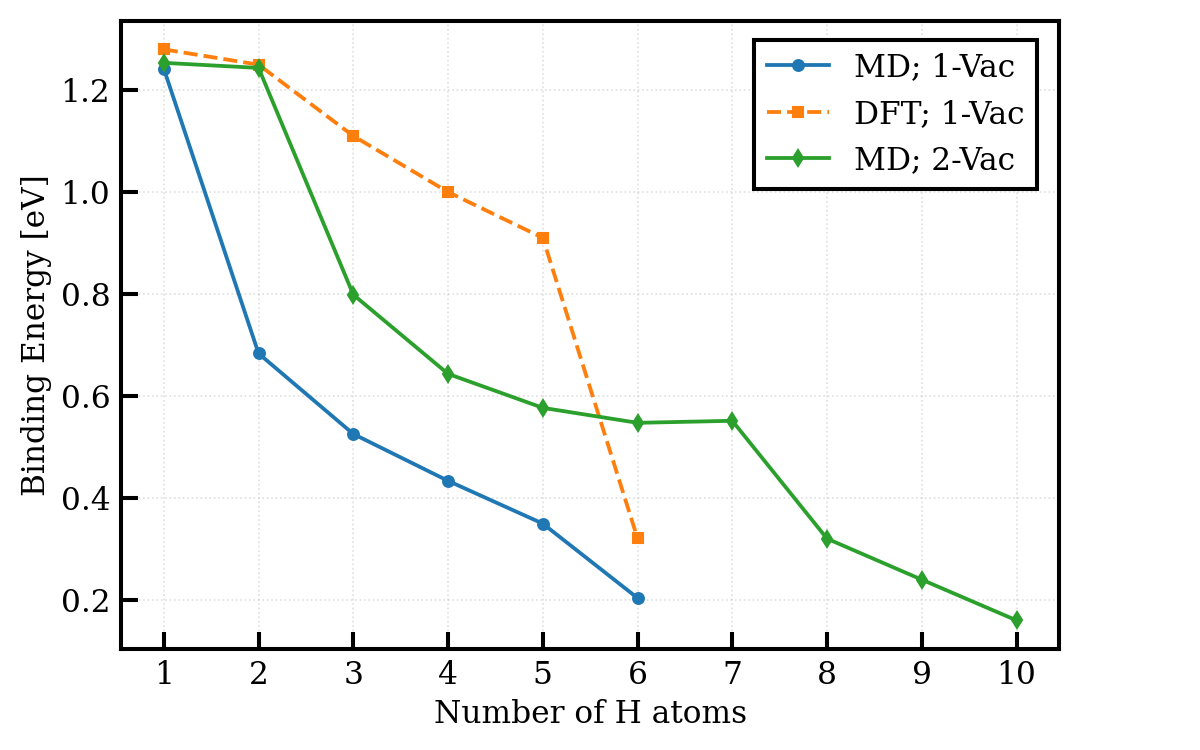
\includegraphics[width=0.5\linewidth]{Ebind.png}
\caption{Comparision of the H-W binding energy in EAM1 by Bonny \textit{et. al} and DFT results by Heinola \textit{et. al. }\cite{heinolaTungstenDFT}}
\label{Fig:Ebind1H_DFT}
\end{figure}

Plotting the potential energy of the individual T atoms as a function of time as in fig. \ref{Fig:Epot}, we can see sharp fluctuations as the atoms move around inside the defect, transitioning in and out of binding energy states.

\begin{figure}[!ht]
\center
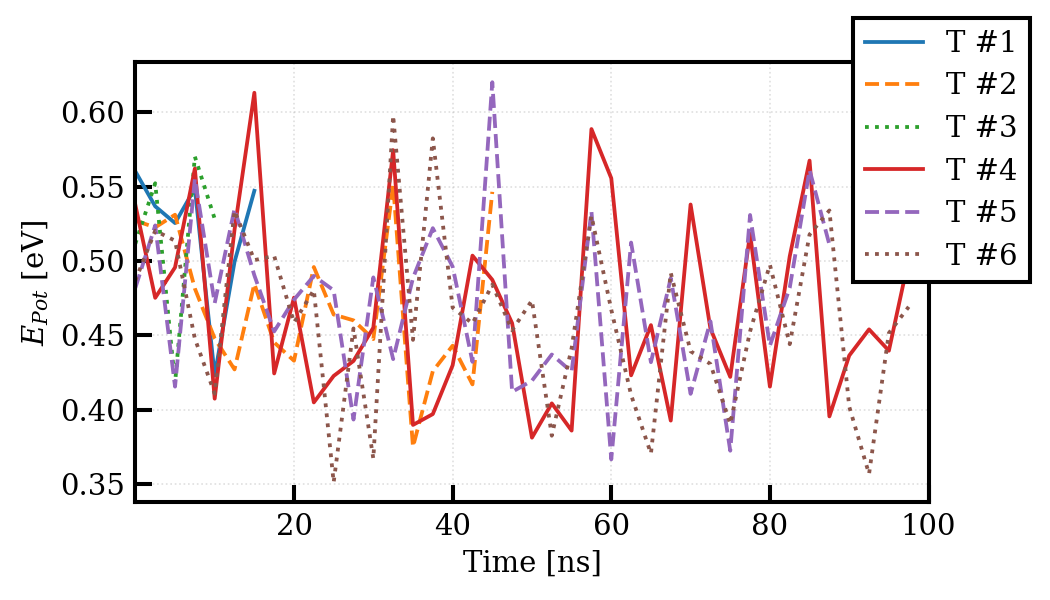
\includegraphics[width=0.52\linewidth]{epot.png}
\caption{The potential energies of all individual T atoms in the 500 K simulation.}
\label{Fig:Epot}
\end{figure}




% ----------------------------------------------------------------------------------
\section{Dislocations}
% ----------------------------------------------------------------------------------
The dislocation results are shown in fig. \ref{Fig:disloc_results}

\begin{figure}[ht]
\begin{subfigure}{.5\textwidth}
  \centering
 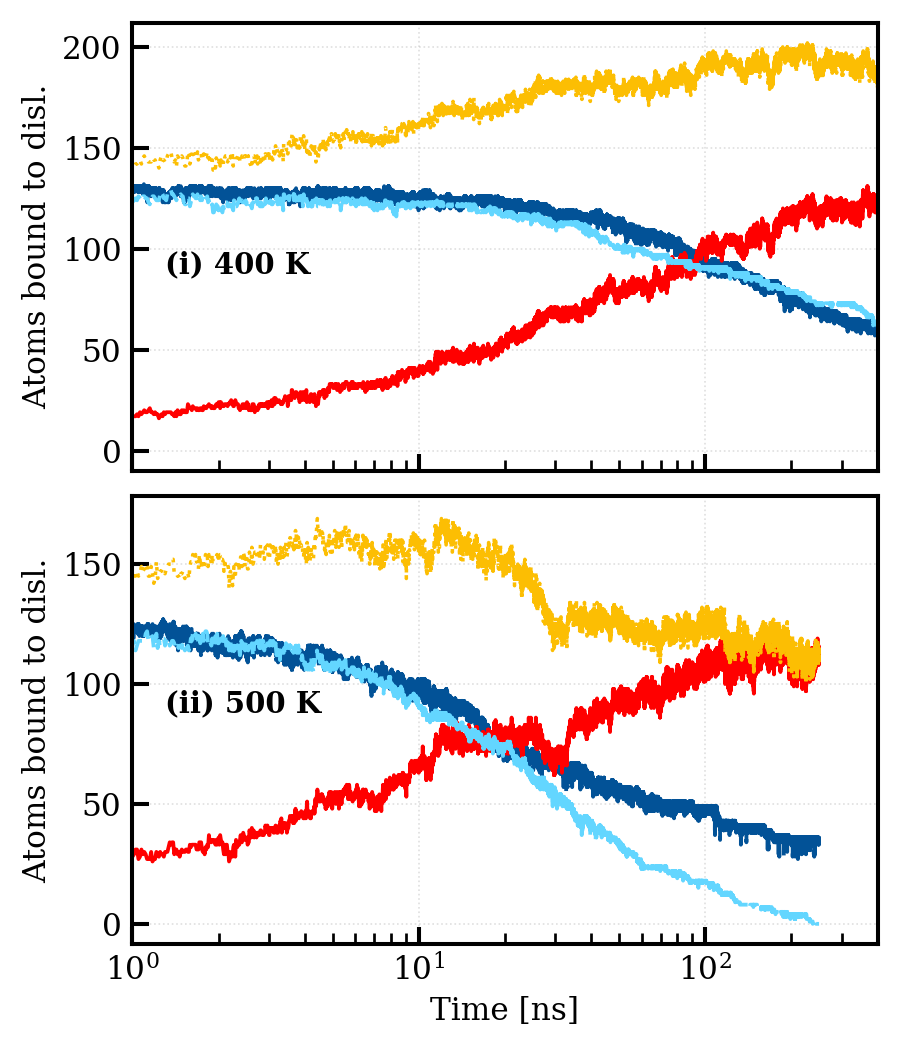
\includegraphics[width=0.99\textwidth]{disloc_isoEx_HT_log.png}  
  \caption{Logarithmic time scale}
  %\label{fig:sub-first}
\end{subfigure}
\begin{subfigure}{.5\textwidth}
  \centering
  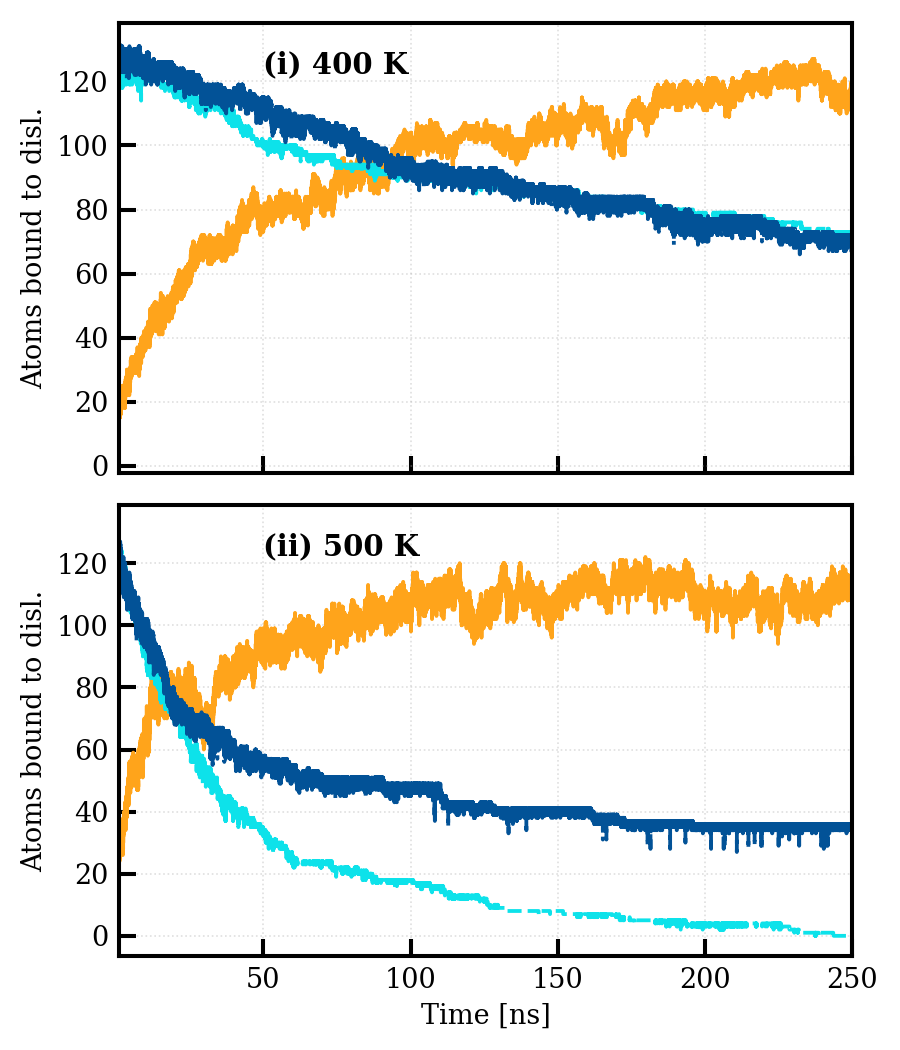
\includegraphics[width=0.99\textwidth]{disloc_isoEx_HT.png}  
  \caption{Linear time scale}
  %\label{fig:sub-second}
\end{subfigure}
   \caption{Number of H and T atoms bound to the dislocation for isotope exchange and diffusion simulations}
   \label{Fig:disloc_results} 
\end{figure}



% ----------------------------------------------------------------------------------
\section{Grain boundaries}
% ----------------------------------------------------------------------------------
The grain boundary results are shown in fig. \ref{Fig:GB_results}

\begin{figure}[ht]
\begin{subfigure}{.5\textwidth}
  \centering
 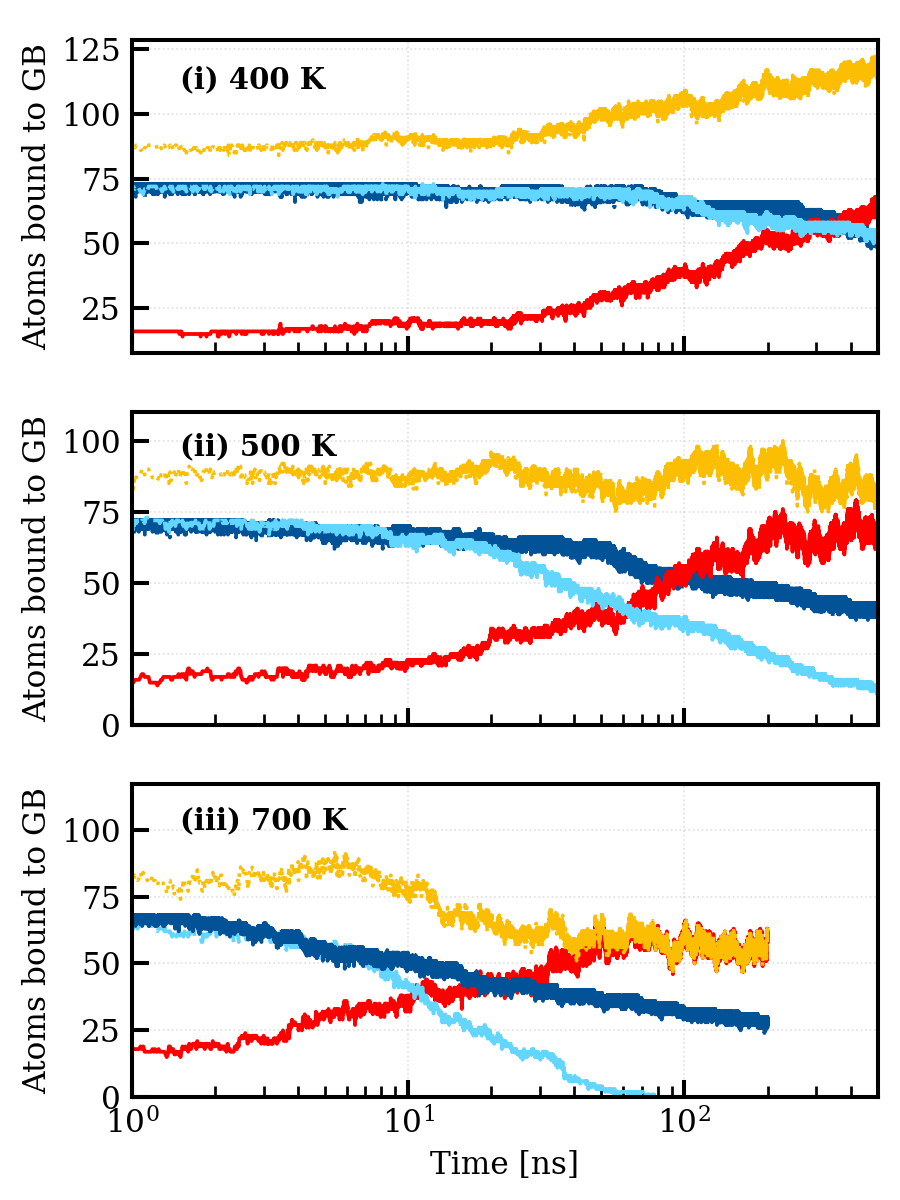
\includegraphics[width=0.99\textwidth]{GB_isoEx_HT_log.png}  
  \caption{Logarithmic time scale}
  %\label{fig:sub-first}
\end{subfigure}
\begin{subfigure}{.5\textwidth}
  \centering
  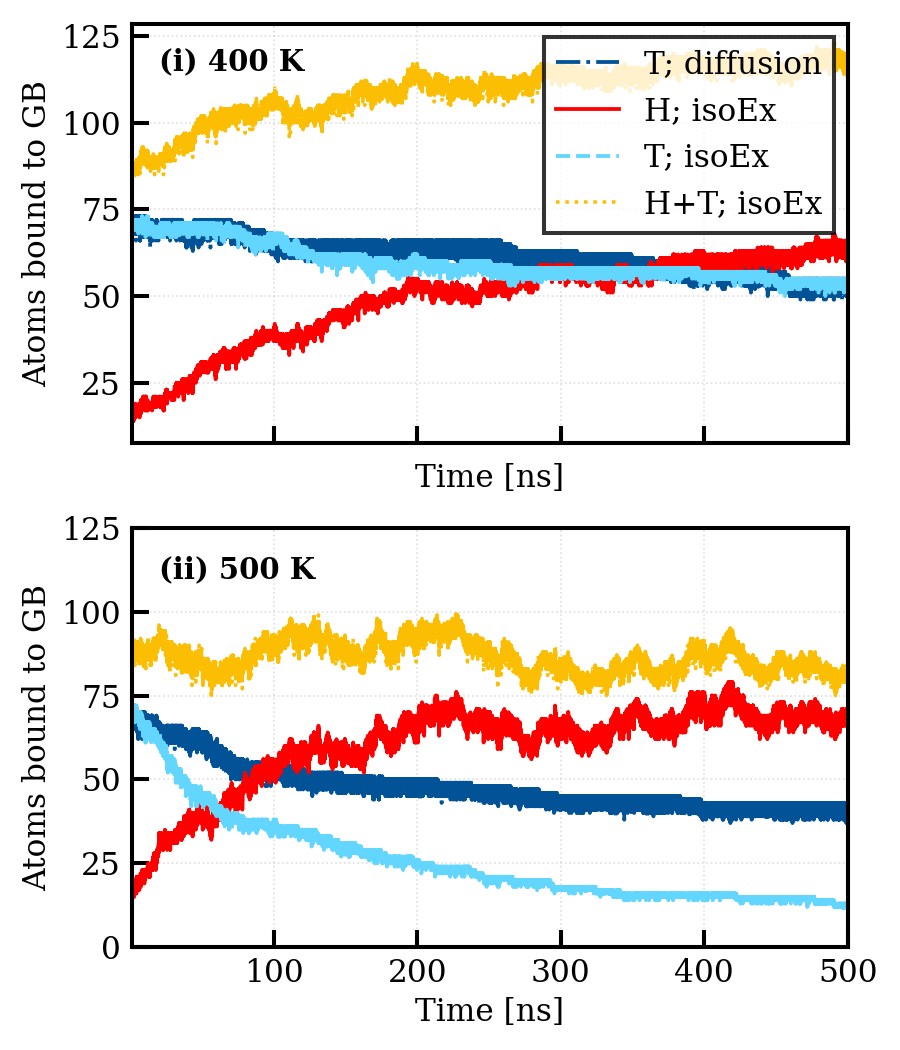
\includegraphics[width=0.99\textwidth]{GB_isoEx_HT.png}  
  \caption{Linear time scale}
  %\label{fig:sub-second}
\end{subfigure}
   \caption{Number of H and T atoms bound to the grain boundary for isotope exchange and diffusion simulations}
   \label{Fig:GB_results} 
\end{figure}

